\documentclass{scrartcl}
 
\usepackage[utf8]{inputenc}
\usepackage[T1]{fontenc}
\usepackage{lmodern}
\usepackage[pdftex]{graphicx}
\usepackage[ngerman]{babel}
\usepackage{amsmath}
\usepackage{amssymb}
\usepackage{tabularx}
\usepackage{multirow}
\usepackage{amsfonts}
\usepackage{tabto}
\usepackage{mathtools}
\TabPositions{0.1in, 0.4in, 0.6in, 0.8in, 1.0in, 1.2in, 3.4in}

\begin{document}
\begin{LARGE}
Spieltheorie - WiSe 2014/15
\end{LARGE}

\begin{Large}
Übungsblatt 8 - Felix Dosch\\[1.0cm]
\end{Large}

\begin{Large}
Aufgabe 8.1\\[0.0cm]
\end{Large}

Abgabe von Java-Code im Anhang.

\begin{itemize}
\item{Gefangenendilemma:  \texttt{FelixDoschPrisonerPlayer.java}}
\end{itemize}
\begin{itemize}
\item{Taube-Falke-Spiel:  \texttt{FelixDoschDoveHawkPlayer.java}}
\end{itemize}

\begin{Large}
Aufgabe 8.2\\[0.0cm]
\end{Large}

Wir benutzen die graphische Methode (wie in Vorlesung 3), um für jeden Spieler den MaxMin-Wert und
damit auch den Wert des Spiels zu bestimmen (endliches zwei-Spieler-Spiel mit perfekter Information
und ohne Zufallsspieler). \\

Spiel A: \\
\begin{figure}[h!]
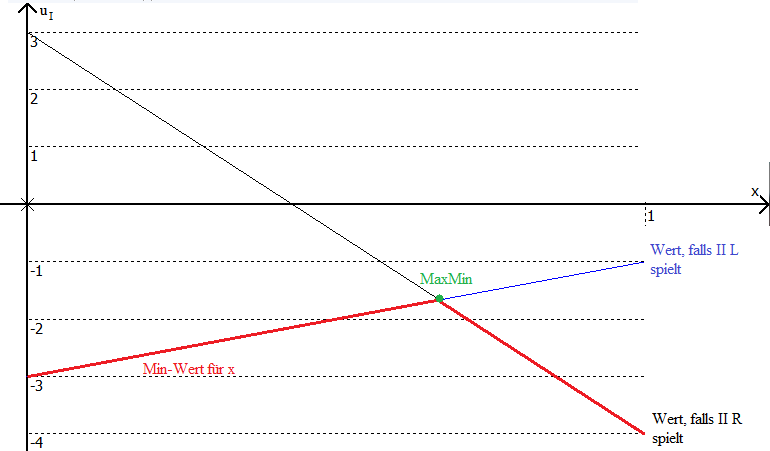
\includegraphics[width=1\textwidth]{2_maxMin_A1.png}
\caption{Wert für Spieler I}
\end{figure}
\begin{figure}
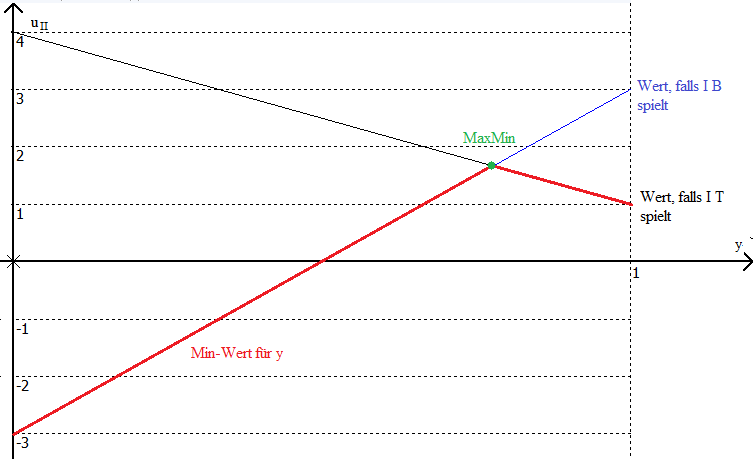
\includegraphics[width=1\textwidth]{2_maxMin_A2.png}
\caption{Wert für Spieler II}
\text{ }\\
Wie sich aus den Abbildungen erkennen lässt, ist der Wert von Spiel A $-\frac{5}{3}$.
\end{figure}
\text{ }\\

\begin{figure}
Spiel B: \\

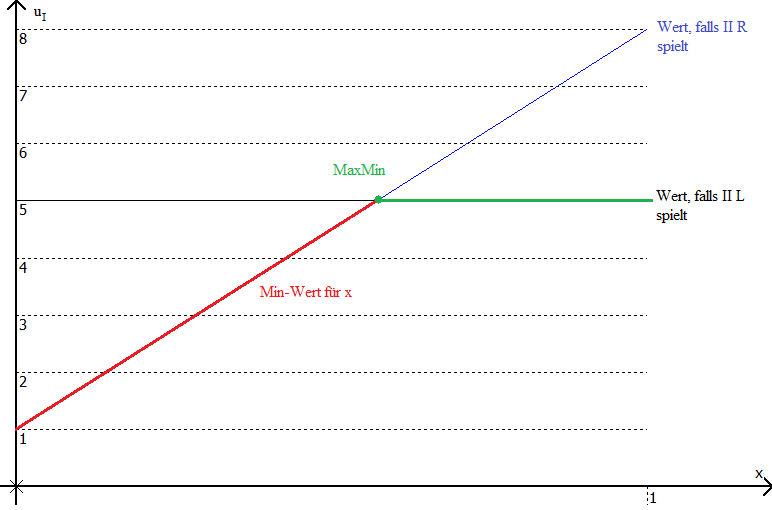
\includegraphics[width=1\textwidth]{2_maxMin_B1.png}
\caption{Wert für Spieler I}
\end{figure}
\begin{figure}
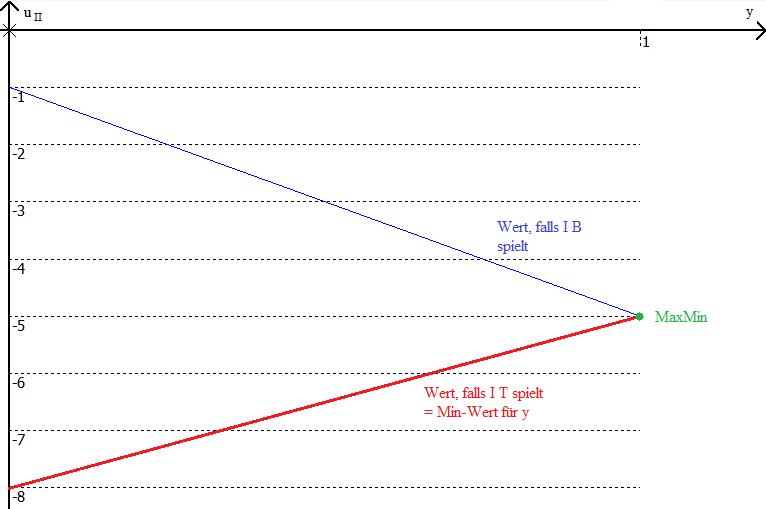
\includegraphics[width=1\textwidth]{2_maxMin_B2.png}
\caption{Wert für Spieler II}
\text{ }\\
Wie sich aus den Abbildungen erkennen lässt, ist der Wert von Spiel B 5.
\end{figure}

\end{document}